\documentclass[12pt,notes]{beamer}
 
\usetheme{FHWN}
\usepackage[utf8]{inputenc}
\usepackage{includes/masterthesis-vars}
\usepackage[UKenglish]{isodate}

\usepackage[group-separator={,}]{siunitx}
\usepackage{supertabular}
\usepackage[nomain,acronym,toc,shortcuts]{glossaries}

\usepackage[backend=bibtex,style=numeric,sorting=anyvt,natbib=true]{biblatex}
\addbibresource{includes/shared-preamble-mainreferences.bib}  %Imports bibliography file
\addbibresource{includes/shared-preamble-tweetreferences.bib} %Imports bibliography file

% the following section is from: https://tex.stackexchange.com/questions/97615/article-style-bibliography-in-beamer-class

% make bibliography entries smaller
\renewcommand\bibfont{\scriptsize}
% If you have more than one page of references, you want to tell beamer
% to put the continuation section label from the second slide onwards
\setbeamertemplate{frametitle continuation}[from second]
% and kill the abominable icon
%\setbeamertemplate{bibliography item}{}
% Now get rid of all the colours
\setbeamercolor*{bibliography entry title}{fg=black}
\setbeamercolor*{bibliography entry author}{fg=black}
\setbeamercolor*{bibliography entry location}{fg=black}
\setbeamercolor*{bibliography entry note}{fg=black}

\newcolumntype{!}{>{\global\let\currentrowstyle\relax}}
\newcolumntype{^}{>{\currentrowstyle}}
\newcommand{\rowstyle}[1]{\gdef\currentrowstyle{#1}%
  #1\ignorespaces
}

\newcommand{\nologo}{\setbeamertemplate{logo}{}} 

\AtBeginSection[]{
  \frame{\tableofcontents[currentsection]}
  % \begin{frame}
  % \vfill
  % \centering
  % \begin{beamercolorbox}[sep=8pt,center,shadow=true,rounded=false]{title}
  %   \usebeamerfont{title}\insertsectionhead\par%
  % \end{beamercolorbox}
  % \vfill
  % \end{frame}
}

\institute{Matriculation No.: \matriculationNumber}
\date{\printdate{2019-06-19}}

\newacronym{EMH}{EMH}{Efficient Market Hypothesis}
\newacronym{ME}{ME}{Maximum Entropy}
\newacronym{NB}{NB}{Naive Bayes}
\newacronym{NLP}{NLP}{Natural Language Processing}
\newacronym{SVM}{SVM}{Support Vector Machines}
\newacronym{TP}{TP}{True Positive}
\newacronym{TN}{TN}{True Negative}
\newacronym{FP}{FP}{False Positive}
\newacronym{FN}{FN}{False Negative}
\newacronym{bow}{bow}{bag of words}
\newacronym{API}{API}{Application Programming Interface}
\newacronym{GB}{GB}{Giga Bytes}
\newacronym{RegEx}{RegEx}{Regular Expression}
\newacronym{TF-IDF}{TF-IDF}{Term Frequency Inverse Document Frequency}
\newacronym{NLTK}{NLTK}{Natural Language Toolkit}
\newacronym{RT}{RT}{retweet}
\newacronym{DMITCAT}{DMI-TCAT}{Digital Methods Initiative Twitter Capture and Analysis Toolset}
\makeglossaries
 
\begin{document}
 
%!TEX root = ../../presentation.tex

\begin{frame}[plain]
    \titlepage
\end{frame}

\begin{frame}
    \frametitle{Table of Contents}
    \tableofcontents
\end{frame}

%!TEX root = ../../presentation.tex

\section{Introduction}
 
\begin{frame}
    \frametitle{Motivation}
    
    \begin{outline}
        \1 Efficient Market Hypothesis (EMH)
        \1 Option Mining
        \1 Twitter as source
    \end{outline}
\end{frame}

\note[itemize]{
    \item EMH: News aren't predictable $\rightarrow$ random walk
    \item New millennium: At least predictable behavioral and psychological elements
    \item Option mining: Big data approach
    \item Why Twitter: Later
}

\begin{frame}
    \frametitle{Research Question}

    \emph{
    To what extent can stock market movements be explained by the public opinion extracted from Twitter?
    }
\end{frame}

\begin{frame}
    \frametitle{Research Goals I}
    
    \begin{outline}
        \1 G1 - Determine companies, keywords and stock symbols to analyze
            \2 Which companies should be analyzed?
            \2 Which keywords should be used to find corresponding tweets?
            \2 Which company uses which stock symbol in order to retrieve share prices?
    \end{outline}
\end{frame}

\begin{frame}
    \frametitle{Research Goals II}

    \begin{outline}

    \1 G2 - Gather tweets and their sentiments and stock prices
        \2 Why Twitter and not any other social media platform?
        \2 In which way can tweets be collected?
        \2 In which way can sentiments be determined?
        \2 Which sentiments are present for various companies?

    \1 G3 - Comparing sentiment time series with share prices
        \2 Can the time series of sentiments explain the share prices?

    \end{outline}
\end{frame}
%!TEX root = ../presentation.tex

\section{Theoretical Background}

\begin{frame}
    \frametitle{Why Twitter?}

    \begin{itemize}
        \item Reliable in previous studies \citep{Barbosa2010}
        \begin{itemize}
            \item Public opinion \citep{Oconnor2010a,Patodkar2016a}
            \item Stock market prediction \citep{Bollen2011a,Mittal2012a,Nguyen2015a,Pagolu2016a,Zhang2011a}
        \end{itemize}

        \item Short messages of up to 280 characters \citep{Rosen2017}
        \item One topic is assumed due limited characters \citep{Pagolu2016a,Patodkar2016a}
    \end{itemize}
\end{frame}
  
\note[itemize]{
    \item Page 11
}

\begin{frame}
    \frametitle{Sentiment Detection Algorithms}

    \begin{itemize}
        \item \tb{}
        \item \nb{}
        \item \me{}
        \item \svm{}
    \end{itemize}
\end{frame}

\note[itemize] {
    \item {
        Naive Bayes:
        \begin{equation}
            P_{NB}(c|d) = \frac{P(c) (\prod_{i=1}^{m} P(f_i|c)^{n_i(d)}) }{P(d)}
            \label{eq:background-optionmining-machinelearningalgorithms-bayes}
        \end{equation}
    }
}

\note[itemize] {
    \item {
     Maximum Entropy:
        \begin{equation}
            P_{ME}(c|d) = \frac{1}{Z(d)} exp \left( \sum_i^m \lambda_{i,c}F_{i,c}(d,c) \right)
            \label{eq:background-optionmining-machinelearningalgorithms-maximumentropy}
        \end{equation}

        \begin{equation}
            Z(d) = \sum_c exp(\sum_i \lambda_{i,c} F_{i,c}(d,c))
            \label{eq:background-optionmining-machinelearningalgorithms-maximumentropy_Zd}
        \end{equation}
    
        \begin{equation}
        F_{i,c}(d,c') = 
            \begin{cases}
            1, & n_i(d) > 0 \text{ and } c' = c \\
            0  & \text{otherwise}
            \end{cases}
            \label{eq:background-optionmining-machinelearningalgorithms-maximumentropy_fic}
        \end{equation}
    }
}

\note[itemize] {
    \item {
        Support Vector Machine:
        \begin{figure}[ht]
            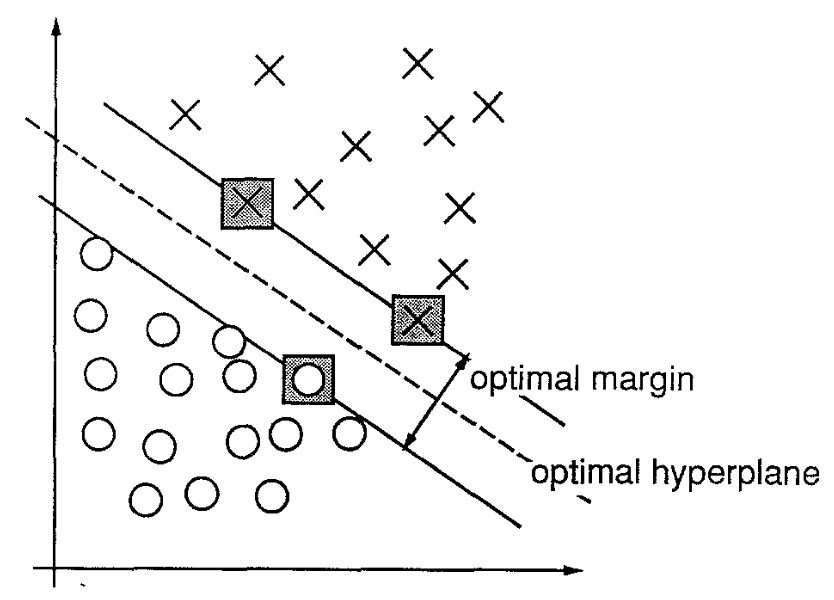
\includegraphics[width=.7\textwidth]{images/svm.png}
            \label{fig:background-optionmining-machinelearningalgorithms-svm}
        \end{figure}        
    }
}
%!TEX root = ../../presentation.tex

\section{Case Study}

\begin{frame}
  \frametitle{Companies \& Keywords}

  \begin{outline}
    \1 Determined five companies
      \2 \ford{}
      \2 \gm{}
      \2 \hyundai{}
      \2 \toyota{}
      \2 \vw{}

    \1 Determined 23 keywords/brands
  \end{outline}
\end{frame}

\note[itemize]{
  \item Table 3.1: Keywords/Brands, page 13-15 (ranking)
  \begin{itemize}
    \item Ford (5)
      \begin{itemize}
        \item Ford, Lincoln
      \end{itemize}

    \item GM (4)
      \begin{itemize}
        \item Baojun, Buick, Cadillac, Chevrolet, GMC, Holden, Jiefang, Wuling
      \end{itemize}

    \item Hyundai (3)
      \begin{itemize}
        \item Hyundai, KIA
      \end{itemize}

    \item Toyota (1)
      \begin{itemize}
        \item Daihatsu, Lexus, Toyota
      \end{itemize}

    \item VW (2)
      \begin{itemize}
        \item Audi, Bentley, Bugatti, Lamborghini, Porsche, Seat, Škoda, Volkswagen
      \end{itemize}

  \end{itemize}
  \item Table 3.2: Five Companies, page 15
}

\begin{frame}
  \frametitle{Stock Symbols}

  {\footnotesize
  \begin{table}
      \centering
      \begin{tabular}[c]{!l ^r ^l ^l}
        \hline
        \rowstyle{\bfseries}
          Company & \#cars\citep{OICA2016} & Market & Symbol  \\ \hline
          \ford{} & 6,429,485 & New York & F  \\
          \gm{} & 7,793,066 & New York & GM \\
          \hyundai{} & 7,889,538 & Korea & 005380.KS \\
          \toyota{} & 10,213,486 & Tokyo & 7203.T \\
          \vw{} & 10,126,281 & Frankfurt & VOW.F \\  \hline
        \end{tabular}
    \end{table}
  }
\end{frame}

\note[itemize]{
  \item Same as Table 3.2: Five Companies, page 15
  \item OICA = Organisation Internationale des Constructeurs d'Automobiles (engl. International Organization of Motor Vehicle Manufacturers)
  \item Daten von dem OICA corresponds survey 2016
}

\begin{frame}
  \frametitle{Gather Data}

  \begin{outline}
    \1 Tweets
      \2 Using DMI-TCAT using Twitter Streaming API
      \2 Gathered Tweets from \printdate{2018-02-28} and \printdate{2018-09-07}
    
    \1 Share Prices
      \2 Yahoo Finance    
  \end{outline}

\end{frame}

\note[itemize]{
  \item Why DMI-TCAT?: page 16/17
  \item Description of datasets beginning with page 24
}

\begin{frame}
  \frametitle{Tweets}

  {\footnotesize
  \begin{table}
      \centering
      \begin{tabular}{!l ^r ^r}
        \hline
        \rowstyle{\bfseries}
            Company     & \# captured tweets  & \# English tweets \\ \hline
            \ford{}     & \num{4518198}       & \num{3745447}     \\
            \gm{}       & \num{575547}        & \num{413817}      \\
            \hyundai{}  & \num{1895306}       & \num{697221}      \\
            \toyota{}   & \num{915868}        & \num{488913}      \\
            \vw{}       & \num{8244083}       & \num{6219350}     \\ \hline
            Total       & \num{16149002}      & \num{11565283}    \\ \hline
      \end{tabular}
    \end{table}
  }
    
\end{frame}
%%!TEX root = ../../presentation.tex

\section{Analysis}
%!TEX root = ../presentation.tex

\section{Conclusion}

\begin{frame}
    \frametitle{Detected Sentiments}

    Positive sentiment ratio by company and classifier

    {\scriptsize
  \begin{table}
      \centering
      \begin{tabular}{!l ^r ^r ^r ^r ^r}
        \hline
        & \tb{} & \nb{} & \me{} & \svm{} & Average \\ 
        \hline
            \ford{} & \SI{87.09}{\percent} & \SI{61.11}{\percent} & \SI{76.96}{\percent} & \SI{73.03}{\percent} & \SI{74.55}{\percent} \\ 
            \gm{} & \SI{90.83}{\percent} & \SI{68.60}{\percent} & \SI{80.26}{\percent} & \SI{80.45}{\percent} & \SI{80.03}{\percent} \\ 
            \hyundai{} & \SI{88.12}{\percent} & \SI{55.05}{\percent} & \SI{77.46}{\percent} & \SI{67.78}{\percent} & \SI{72.10}{\percent} \\ 
            \toyota{} & \SI{87.86}{\percent} & \SI{55.45}{\percent} & \SI{81.12}{\percent} & \SI{80.11}{\percent} & \SI{76.13}{\percent} \\ 
            \vw{} & \SI{85.20}{\percent} & \SI{47.97}{\percent} & \SI{68.26}{\percent} & \SI{64.58}{\percent} & \SI{66.50}{\percent} \\ \hline
            Average & \SI{87.82}{\percent} & \SI{57.63}{\percent} & \SI{76.81}{\percent} & \SI{73.19}{\percent} & \SI{73.86}{\percent} \\
        \hline
        \end{tabular}
    \end{table}
  }
\end{frame}

\begin{frame}
    \frametitle{Conclusion I}

    

\end{frame}
%!TEX root = ../../presentation.tex

\begin{frame}[allowframebreaks]
    \frametitle{References}
    \printbibliography[title={References}]
\end{frame}
 
\end{document}